\documentclass{standalone}

% Packages
\usepackage{pst-sigsys}
\usepackage{tikz}
\usetikzlibrary{arrows}

% Commands
\newcommand*\circled[1]{\tikz[baseline=(char.base)]{
            \node[shape=circle,draw,inner sep=2pt] (char) {#1};}}

\newcommand{\midarrow}{\tikz \draw[-triangle 90] (0,0) -- +(.1,0);}

\begin{document}
    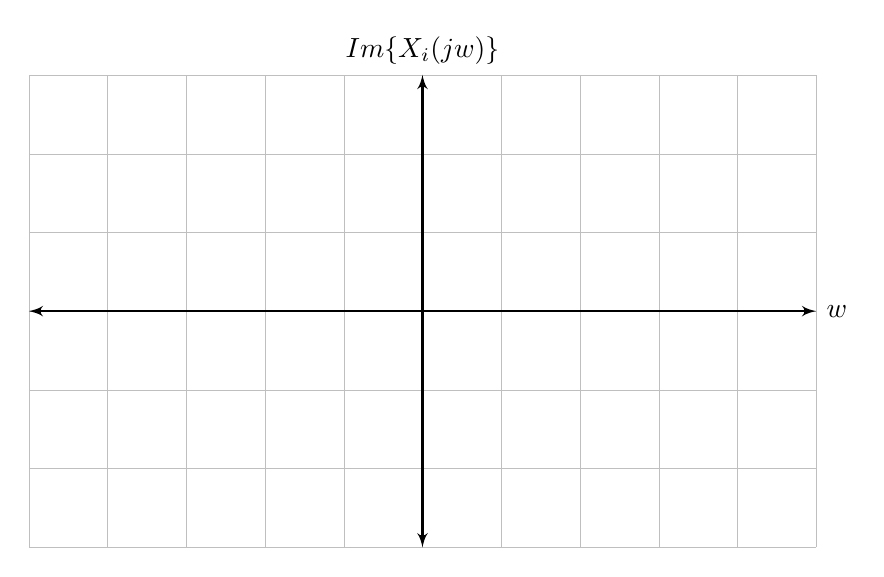
\begin{tikzpicture}[>=latex']
    \draw[lightgray, ultra thin] (-5,-3) grid (5,3);
    \draw[thick,<->] (-5,0) -- (5,0) node [anchor=west] {$w$};
    \draw[thick,<->] (0,-3) -- (0,3) node [anchor=south] {$Im\{\textrm{$X_i$}(jw)\}$};
    \end{tikzpicture}
\end{document}
